\documentclass[11pt]{article}

\usepackage[utf8]{inputenc}
\usepackage[T1]{fontenc}
\usepackage{lmodern}
\usepackage{amsmath,amssymb,amsfonts}
\usepackage{graphicx}
\usepackage{booktabs}
\usepackage{caption}
\usepackage{subcaption}
\usepackage{makecell}
\usepackage{booktabs}
\usepackage{algorithm}
\usepackage{algpseudocode}


\usepackage{tikz}
\usetikzlibrary{arrows.meta}
\usepackage{xcolor}
\definecolor{origincolor}{RGB}{72, 175, 130}
\definecolor{destcolor}{RGB}{210, 90, 70}
\definecolor{intcolor}{RGB}{150, 150, 150}
\definecolor{auxcolor}{RGB}{180, 180, 180}
\definecolor{crossgreen}{RGB}{29, 158, 117}
\definecolor{crosspurple}{RGB}{120, 100, 200}
\definecolor{crossyellow}{RGB}{200, 140, 0}
\DeclareMathOperator*{\argmax}{arg\,max}


\DeclareMathOperator*{\argmin}{arg\,min}

\usepackage{geometry}
\geometry{margin=1in}

\usepackage{setspace}
\onehalfspacing

\usepackage{hyperref}
\hypersetup{
    colorlinks=true,
    linkcolor=blue,
    citecolor=blue,
    urlcolor=blue
}

\usepackage[
    backend=biber,
    style=authoryear,
    sorting=ynt
]{biblatex}
\addbibresource{sample.bib}


\title{Graph Multi-Output Gaussian Processes for Origin-Destination Matrix Calibration via Bayesian Optimization}



\author{Inès Ben Hamza}
\date{June 2026}

\begin{document}


\section{Networks}
% ,,,,,,,,,,,,,,,,,,,,
\subsection{Toy Network (two-corridor)}
\label{app:network_toy}
% ,,,,,,,,,,,,,,,,,,,,


\subsubsection*{Topology}

The \emph{quickstart} toy network is a two-corridor graph with two origin TAZs
(91, 92) and two destination TAZs (93, 94), connected through six internal
junctions (1--6) and four intermediate single-degree auxiliary nodes
(911--914). The cross-links \texttt{L15} ($6 \to 3$) and \texttt{L16}
($3 \to 6$) couple the two corridors. 
Figure~\ref{fig:network-toy-detail} shows all raw SUMO edge IDs;
Figure~\ref{fig:network_toy} shows the same network after edge grouping, which
yields \textbf{6 grouped flow variables}, \textbf{4 OD pairs}, and \textbf{4
routes} in total.

\begin{figure}[ht]
\centering
\resizebox{\textwidth}{!}{%
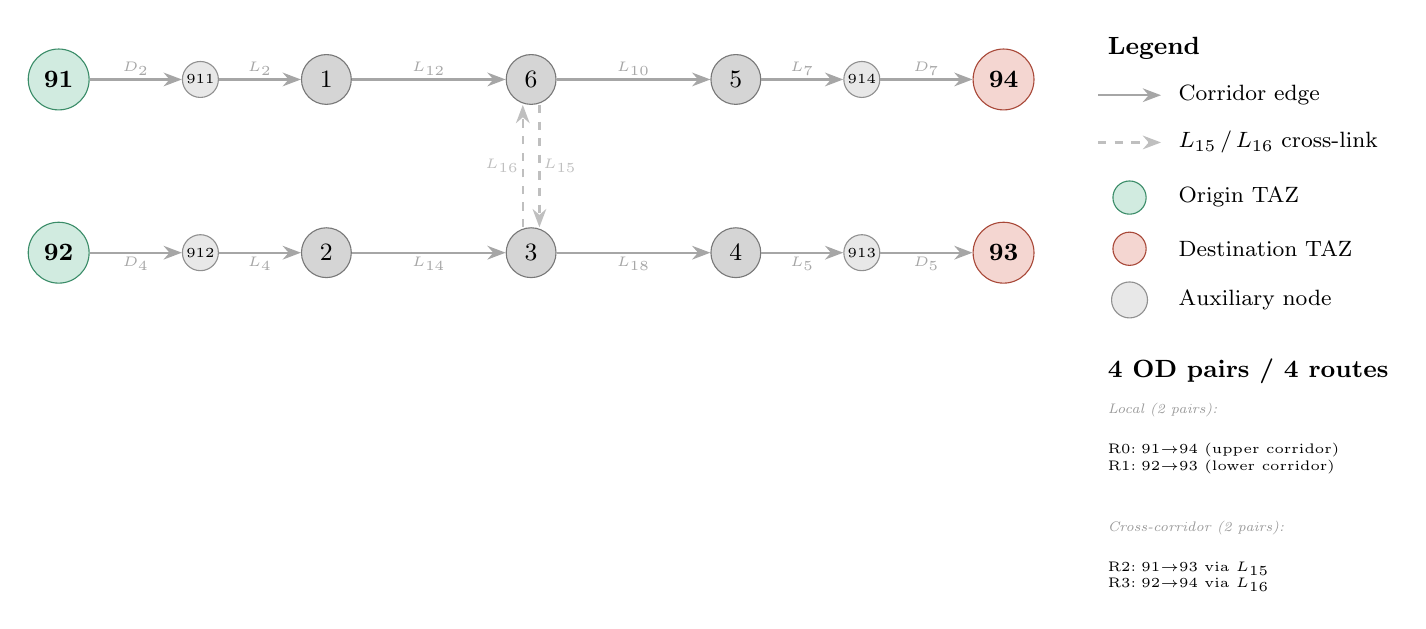
\begin{tikzpicture}[
    >=Stealth,
    onode/.style  = {circle, draw=origincolor!80!black, fill=origincolor!25,
                     minimum size=22pt, inner sep=0pt, font=\small\bfseries},
    dnode/.style  = {circle, draw=destcolor!80!black,   fill=destcolor!25,
                     minimum size=22pt, inner sep=0pt, font=\small\bfseries},
    inode/.style  = {circle, draw=intcolor!80!black,    fill=intcolor!40,
                     minimum size=18pt, inner sep=0pt, font=\small},
    anode/.style  = {circle, draw=auxcolor!80!black,    fill=auxcolor!30,
                     minimum size=13pt, inner sep=0pt, font=\tiny},
    fwd/.style    = {->, thick, gray!70},
    lbl/.style    = {font=\tiny, inner sep=1pt},
]
%% Upper corridor
\node[onode](n91)  at( 0.0,  0.0){91};
\node[anode](a911) at( 1.8,  0.0){\tiny 911};
\node[inode](n1)   at( 3.4,  0.0){1};
\node[inode](n6)   at( 6.0,  0.0){6};
\node[inode](n5)   at( 8.6,  0.0){5};
\node[anode](a914) at(10.2,  0.0){\tiny 914};
\node[dnode](n94)  at(12.0,  0.0){94};
%% Lower corridor
\node[onode](n92)  at( 0.0, -2.2){92};
\node[anode](a912) at( 1.8, -2.2){\tiny 912};
\node[inode](n2)   at( 3.4, -2.2){2};
\node[inode](n3)   at( 6.0, -2.2){3};
\node[inode](n4)   at( 8.6, -2.2){4};
\node[anode](a913) at(10.2, -2.2){\tiny 913};
\node[dnode](n93)  at(12.0, -2.2){93};
%% Upper corridor edges
\draw[fwd](n91)--node[lbl,above]{$D_2$}(a911);
\draw[fwd](a911)--node[lbl,above]{$L_2$}(n1);
\draw[fwd](n1)--node[lbl,above]{$L_{12}$}(n6);
\draw[fwd](n6)--node[lbl,above]{$L_{10}$}(n5);
\draw[fwd](n5)--node[lbl,above]{$L_7$}(a914);
\draw[fwd](a914)--node[lbl,above]{$D_7$}(n94);
%% Lower corridor edges
\draw[fwd](n92)--node[lbl,below]{$D_4$}(a912);
\draw[fwd](a912)--node[lbl,below]{$L_4$}(n2);
\draw[fwd](n2)--node[lbl,below]{$L_{14}$}(n3);
\draw[fwd](n3)--node[lbl,below]{$L_{18}$}(n4);
\draw[fwd](n4)--node[lbl,below]{$L_5$}(a913);
\draw[fwd](a913)--node[lbl,below]{$D_5$}(n93);
%% Cross links
\draw[->,thick,gray!50,dashed]([xshift= 3pt]n6.south)--
    node[lbl,right]{$L_{15}$}([xshift= 3pt]n3.north);
\draw[->,thick,gray!50,dashed]([xshift=-3pt]n3.north)--
    node[lbl,left]{$L_{16}$}([xshift=-3pt]n6.south);
%% Legend + OD table
\begin{scope}[shift={(13.2, 0.4)}]
    \node[font=\small\bfseries,anchor=west]at(0,0){Legend};
    \draw[fwd](0,-0.6)--(0.8,-0.6);
    \node[font=\footnotesize,anchor=west]at(0.9,-0.6){Corridor edge};
    \draw[->,thick,gray!50,dashed](0,-1.2)--(0.8,-1.2);
    \node[font=\footnotesize,anchor=west]at(0.9,-1.2){$L_{15}$\,/\,$L_{16}$ cross-link};
    \node[onode,minimum size=12pt]at(0.4,-1.9){};
    \node[font=\footnotesize,anchor=west]at(0.9,-1.9){Origin TAZ};
    \node[dnode,minimum size=12pt]at(0.4,-2.55){};
    \node[font=\footnotesize,anchor=west]at(0.9,-2.55){Destination TAZ};
    \node[anode]at(0.4,-3.2){};
    \node[font=\footnotesize,anchor=west]at(0.9,-3.2){Auxiliary node};
    \node[font=\small\bfseries,anchor=west]at(0,-4.1){4 OD pairs / 4 routes};
    \node[font=\tiny,text=gray!80,anchor=west]at(0,-4.6){\textit{Local (2 pairs):}};
    \node[font=\tiny,anchor=north west,align=left]at(0,-4.9){%
        R0:\;$91{\to}94$ (upper corridor)\\
        R1:\;$92{\to}93$ (lower corridor)};
    \node[font=\tiny,text=gray!80,anchor=west]at(0,-6.1){\textit{Cross-corridor (2 pairs):}};
    \node[font=\tiny,anchor=north west,align=left]at(0,-6.4){%
        R2:\;$91{\to}93$ via $L_{15}$\\
        R3:\;$92{\to}94$ via $L_{16}$};
\end{scope}
\end{tikzpicture}%
}
\caption{Toy network with all raw SUMO edge IDs. Auxiliary nodes 911--914 are
single-degree merge points that carry identical flow to their adjacent edge and are
therefore absorbed into grouped flow variables (see Figure~\ref{fig:network_toy}).}
\label{fig:network-toy-detail}
\end{figure}

\begin{figure}[h]
\centering
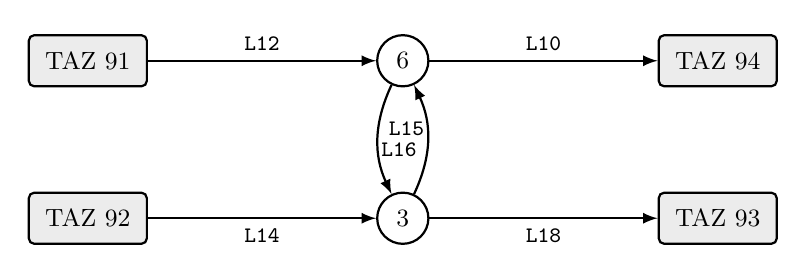
\begin{tikzpicture}[
    taz/.style   = {rectangle, draw, fill=gray!15, rounded corners=2pt,
                    minimum width=1.5cm, minimum height=0.65cm,
                    font=\small},
    junc/.style  = {circle, draw, fill=white, minimum size=0.65cm, font=\small},
    grp/.style   = {font=\footnotesize, midway},
    >=latex, thick
]
  %% Only junctions 6 and 3 survive grouping; 1,2,4,5,911-914 are absorbed.
  \node[taz]  (t91) at (0,2)   {TAZ 91};
  \node[junc] (j6)  at (4,2)   {6};
  \node[taz]  (t94) at (8,2)   {TAZ 94};

  \node[taz]  (t92) at (0,0)   {TAZ 92};
  \node[junc] (j3)  at (4,0)   {3};
  \node[taz]  (t93) at (8,0)   {TAZ 93};

  \draw[->] (t91) -- node[grp, above]{\texttt{L12}} (j6);
  \draw[->] (j6)  -- node[grp, above]{\texttt{L10}} (t94);
  \draw[->] (t92) -- node[grp, below]{\texttt{L14}} (j3);
  \draw[->] (j3)  -- node[grp, below]{\texttt{L18}} (t93);

  \draw[->, bend right=25] (j6) to
      node[right, font=\footnotesize, pos=0.4]{\texttt{L15}} (j3);
  \draw[->, bend right=25] (j3) to
      node[left,  font=\footnotesize, pos=0.4]{\texttt{L16}} (j6);
\end{tikzpicture}
\caption{Toy network after edge grouping. Each group collapses a chain of raw edges
into a single flow variable: \texttt{L12} = \{D2, L2, L12\}, \texttt{L10} = \{D7, L7, L10\},
\texttt{L14} = \{D4, L4, L14\}, \texttt{L18} = \{D5, L5, L18\}.
Intermediate junctions (1, 2, 4, 5) and auxiliary nodes (911--914) are absorbed
and no longer appear.}
\label{fig:network_toy}
\end{figure}


%%%%%%%%%%%%%%%%%%%%%%%%%%%%%%%%%%
%%%%%%%%%%%%%%%%%%%%%%%%%%
\subsection{Scaled Network (\texttt{quickstart\_grid\_3})}
\label{app:network_grid3}

\subsubsection*{Topology}

The \texttt{quickstart\_grid\_3} network is constructed by replicating the
two-corridor base module three times (copies 0, 1, 2) and connecting adjacent
copies at their left and right interior junctions via bidirectional
\emph{green} and \emph{purple} cross-streets
(Figure~\ref{fig:network-grid3}). This yields 6 origin TAZs, 6 destination
TAZs, \textbf{36 grouped flow variables}, \textbf{16 OD pairs}, and
\textbf{20 routes} in total.

\begin{figure}[ht]
\centering
\resizebox{\textwidth}{!}{%
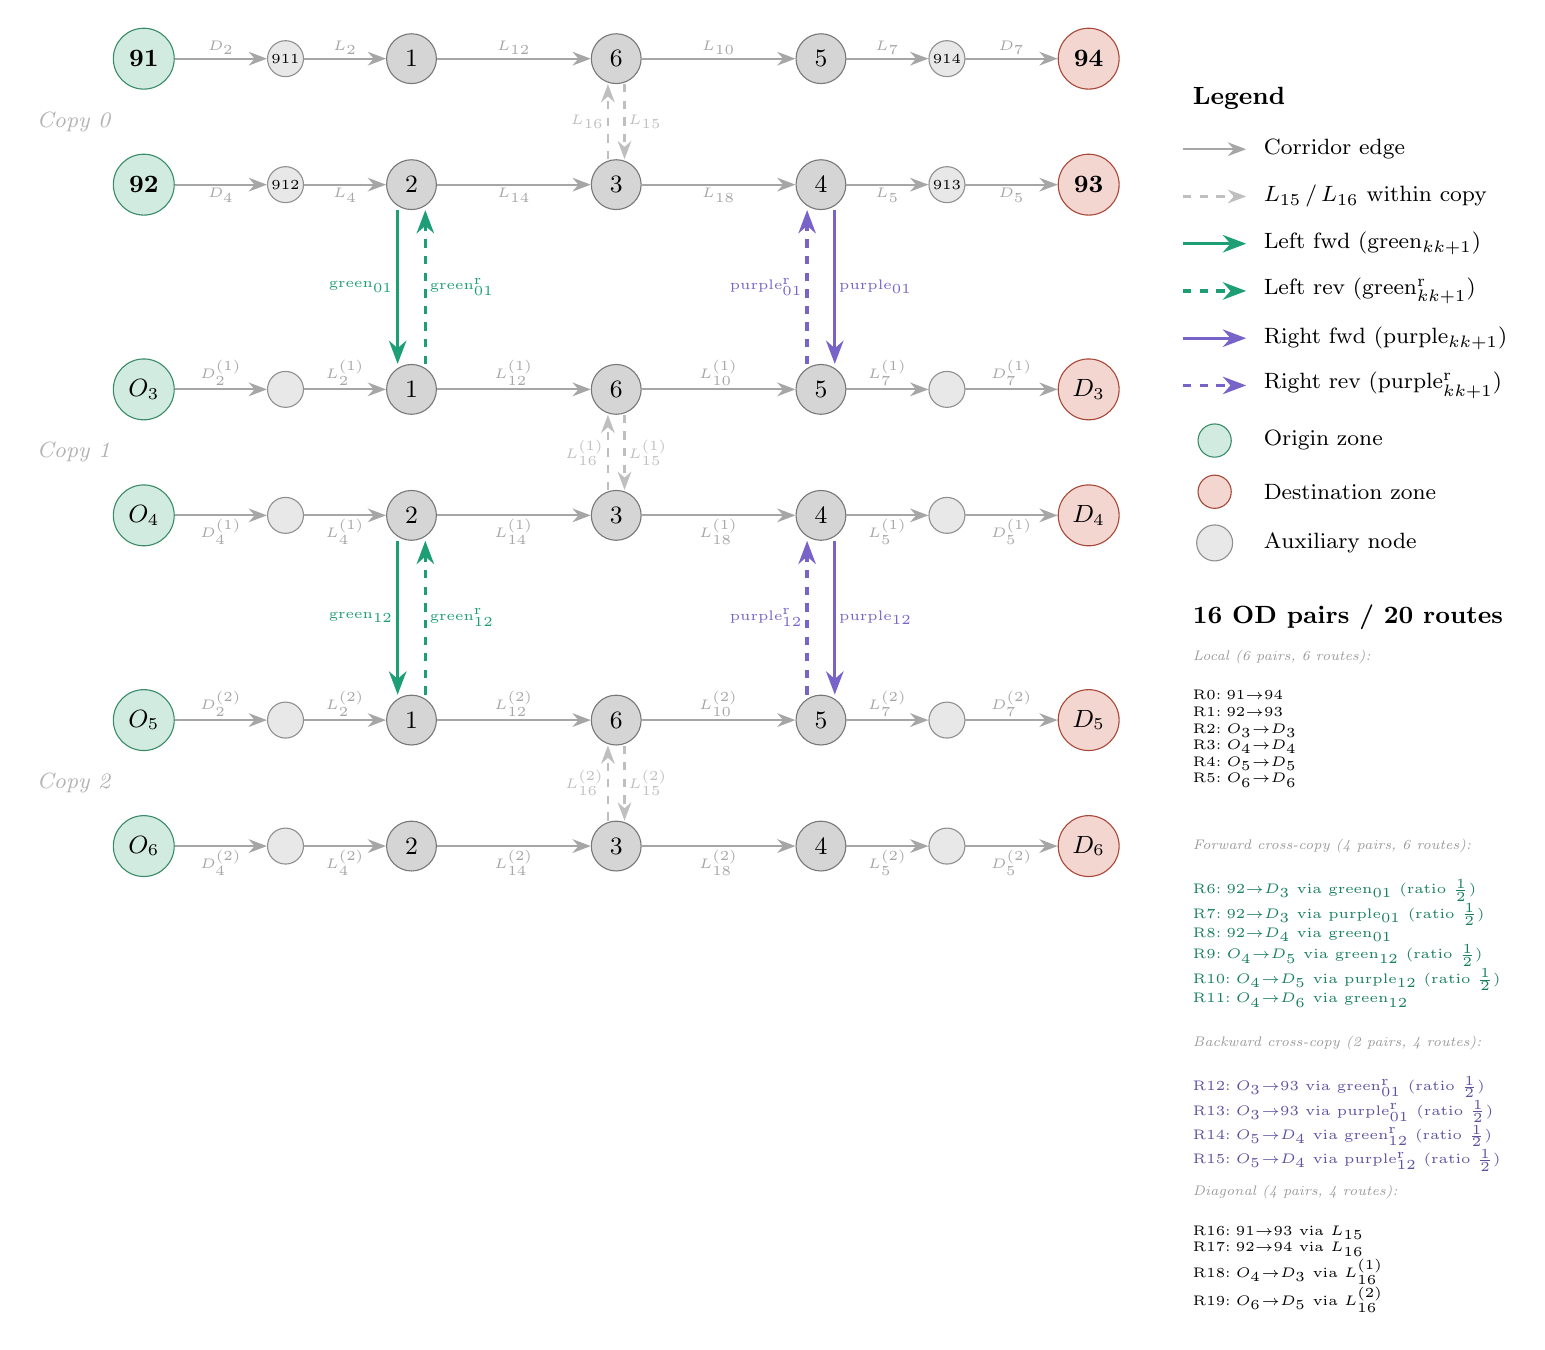
\begin{tikzpicture}[
    >=Stealth,
    onode/.style  = {circle, draw=origincolor!80!black, fill=origincolor!25,
                     minimum size=22pt, inner sep=0pt, font=\small\bfseries},
    dnode/.style  = {circle, draw=destcolor!80!black,   fill=destcolor!25,
                     minimum size=22pt, inner sep=0pt, font=\small\bfseries},
    inode/.style  = {circle, draw=intcolor!80!black,    fill=intcolor!40,
                     minimum size=18pt, inner sep=0pt, font=\small},
    anode/.style  = {circle, draw=auxcolor!80!black,    fill=auxcolor!30,
                     minimum size=13pt, inner sep=0pt, font=\tiny},
    fwd/.style    = {->, thick, gray!70},
    lbl/.style    = {font=\tiny, inner sep=1pt},
    gfwd/.style   = {->, very thick, crossgreen},
    pfwd/.style   = {->, very thick, crosspurple},
    grev/.style   = {->, very thick, crossgreen,  dashed},
    prev/.style   = {->, very thick, crosspurple, dashed},
]

%% ===== NODES =====

%% Copy 0
\node[onode](91)  at( 0.0,  0.0){91};  \node[anode](a91) at( 1.8,  0.0){\tiny 911};
\node[inode](1c0) at( 3.4,  0.0){1};   \node[inode](6c0) at( 6.0,  0.0){6};
\node[inode](5c0) at( 8.6,  0.0){5};   \node[anode](a94) at(10.2,  0.0){\tiny 914};
\node[dnode](94)  at(12.0,  0.0){94};

\node[onode](92)  at( 0.0, -1.6){92};  \node[anode](a92) at( 1.8, -1.6){\tiny 912};
\node[inode](2c0) at( 3.4, -1.6){2};   \node[inode](3c0) at( 6.0, -1.6){3};
\node[inode](4c0) at( 8.6, -1.6){4};   \node[anode](a93) at(10.2, -1.6){\tiny 913};
\node[dnode](93)  at(12.0, -1.6){93};

%% Copy 1
\node[onode](O3)  at( 0.0, -4.2){$O_3$}; \node[anode](a1t1) at( 1.8, -4.2){};
\node[inode](1c1) at( 3.4, -4.2){1};      \node[inode](6c1)  at( 6.0, -4.2){6};
\node[inode](5c1) at( 8.6, -4.2){5};      \node[anode](a1r1) at(10.2, -4.2){};
\node[dnode](D3)  at(12.0, -4.2){$D_3$};

\node[onode](O4)  at( 0.0, -5.8){$O_4$}; \node[anode](a1b1) at( 1.8, -5.8){};
\node[inode](2c1) at( 3.4, -5.8){2};      \node[inode](3c1)  at( 6.0, -5.8){3};
\node[inode](4c1) at( 8.6, -5.8){4};      \node[anode](a1b2) at(10.2, -5.8){};
\node[dnode](D4)  at(12.0, -5.8){$D_4$};

%% Copy 2
\node[onode](O5)  at( 0.0, -8.4){$O_5$}; \node[anode](a2t1) at( 1.8, -8.4){};
\node[inode](1c2) at( 3.4, -8.4){1};      \node[inode](6c2)  at( 6.0, -8.4){6};
\node[inode](5c2) at( 8.6, -8.4){5};      \node[anode](a2r1) at(10.2, -8.4){};
\node[dnode](D5)  at(12.0, -8.4){$D_5$};

\node[onode](O6)  at( 0.0,-10.0){$O_6$}; \node[anode](a2b1) at( 1.8,-10.0){};
\node[inode](2c2) at( 3.4,-10.0){2};      \node[inode](3c2)  at( 6.0,-10.0){3};
\node[inode](4c2) at( 8.6,-10.0){4};      \node[anode](a2b2) at(10.2,-10.0){};
\node[dnode](D6)  at(12.0,-10.0){$D_6$};

%%=============================================================
%%  CORRIDOR EDGES
%%=============================================================

%% Copy 0 — top
\draw[fwd](91) --node[lbl,above]{$D_2$}(a91);
\draw[fwd](a91)--node[lbl,above]{$L_2$}(1c0);
\draw[fwd](1c0)--node[lbl,above]{$L_{12}$}(6c0);
\draw[fwd](6c0)--node[lbl,above]{$L_{10}$}(5c0);
\draw[fwd](5c0)--node[lbl,above]{$L_7$}(a94);
\draw[fwd](a94)--node[lbl,above]{$D_7$}(94);
%% Copy 0 — bottom
\draw[fwd](92) --node[lbl,below]{$D_4$}(a92);
\draw[fwd](a92)--node[lbl,below]{$L_4$}(2c0);
\draw[fwd](2c0)--node[lbl,below]{$L_{14}$}(3c0);
\draw[fwd](3c0)--node[lbl,below]{$L_{18}$}(4c0);
\draw[fwd](4c0)--node[lbl,below]{$L_5$}(a93);
\draw[fwd](a93)--node[lbl,below]{$D_5$}(93);
%% Copy 0 — L15/L16
\draw[->,thick,gray!50,dashed]([xshift= 3pt]6c0.south)--
    node[lbl,right]{$L_{15}$}([xshift= 3pt]3c0.north);
\draw[->,thick,gray!50,dashed]([xshift=-3pt]3c0.north)--
    node[lbl,left]{$L_{16}$}([xshift=-3pt]6c0.south);

%% Copy 1 — top
\draw[fwd](O3) --node[lbl,above]{$D_2^{(1)}$}(a1t1);
\draw[fwd](a1t1)--node[lbl,above]{$L_2^{(1)}$}(1c1);
\draw[fwd](1c1)--node[lbl,above]{$L_{12}^{(1)}$}(6c1);
\draw[fwd](6c1)--node[lbl,above]{$L_{10}^{(1)}$}(5c1);
\draw[fwd](5c1)--node[lbl,above]{$L_7^{(1)}$}(a1r1);
\draw[fwd](a1r1)--node[lbl,above]{$D_7^{(1)}$}(D3);
%% Copy 1 — bottom
\draw[fwd](O4) --node[lbl,below]{$D_4^{(1)}$}(a1b1);
\draw[fwd](a1b1)--node[lbl,below]{$L_4^{(1)}$}(2c1);
\draw[fwd](2c1)--node[lbl,below]{$L_{14}^{(1)}$}(3c1);
\draw[fwd](3c1)--node[lbl,below]{$L_{18}^{(1)}$}(4c1);
\draw[fwd](4c1)--node[lbl,below]{$L_5^{(1)}$}(a1b2);
\draw[fwd](a1b2)--node[lbl,below]{$D_5^{(1)}$}(D4);
%% Copy 1 — L15/L16
\draw[->,thick,gray!50,dashed]([xshift= 3pt]6c1.south)--
    node[lbl,right]{$L_{15}^{(1)}$}([xshift= 3pt]3c1.north);
\draw[->,thick,gray!50,dashed]([xshift=-3pt]3c1.north)--
    node[lbl,left]{$L_{16}^{(1)}$}([xshift=-3pt]6c1.south);

%% Copy 2 — top
\draw[fwd](O5) --node[lbl,above]{$D_2^{(2)}$}(a2t1);
\draw[fwd](a2t1)--node[lbl,above]{$L_2^{(2)}$}(1c2);
\draw[fwd](1c2)--node[lbl,above]{$L_{12}^{(2)}$}(6c2);
\draw[fwd](6c2)--node[lbl,above]{$L_{10}^{(2)}$}(5c2);
\draw[fwd](5c2)--node[lbl,above]{$L_7^{(2)}$}(a2r1);
\draw[fwd](a2r1)--node[lbl,above]{$D_7^{(2)}$}(D5);
%% Copy 2 — bottom
\draw[fwd](O6) --node[lbl,below]{$D_4^{(2)}$}(a2b1);
\draw[fwd](a2b1)--node[lbl,below]{$L_4^{(2)}$}(2c2);
\draw[fwd](2c2)--node[lbl,below]{$L_{14}^{(2)}$}(3c2);
\draw[fwd](3c2)--node[lbl,below]{$L_{18}^{(2)}$}(4c2);
\draw[fwd](4c2)--node[lbl,below]{$L_5^{(2)}$}(a2b2);
\draw[fwd](a2b2)--node[lbl,below]{$D_5^{(2)}$}(D6);
%% Copy 2 — L15/L16
\draw[->,thick,gray!50,dashed]([xshift= 3pt]6c2.south)--
    node[lbl,right]{$L_{15}^{(2)}$}([xshift= 3pt]3c2.north);
\draw[->,thick,gray!50,dashed]([xshift=-3pt]3c2.north)--
    node[lbl,left]{$L_{16}^{(2)}$}([xshift=-3pt]6c2.south);

%%=============================================================
%%  INTER-COPY LINKS
%%=============================================================

\draw[gfwd]([xshift=-5pt]2c0.south)--
    node[lbl,left,text=crossgreen]{$\mathrm{green}_{01}$}
    ([xshift=-5pt]1c1.north);
\draw[grev]([xshift=5pt]1c1.north)--
    node[lbl,right,text=crossgreen]{$\mathrm{green}_{01}^{\mathrm{r}}$}
    ([xshift=5pt]2c0.south);

\draw[gfwd]([xshift=-5pt]2c1.south)--
    node[lbl,left,text=crossgreen]{$\mathrm{green}_{12}$}
    ([xshift=-5pt]1c2.north);
\draw[grev]([xshift=5pt]1c2.north)--
    node[lbl,right,text=crossgreen]{$\mathrm{green}_{12}^{\mathrm{r}}$}
    ([xshift=5pt]2c1.south);

\draw[pfwd]([xshift=5pt]4c0.south)--
    node[lbl,right,text=crosspurple]{$\mathrm{purple}_{01}$}
    ([xshift=5pt]5c1.north);
\draw[prev]([xshift=-5pt]5c1.north)--
    node[lbl,left,text=crosspurple]{$\mathrm{purple}_{01}^{\mathrm{r}}$}
    ([xshift=-5pt]4c0.south);

\draw[pfwd]([xshift=5pt]4c1.south)--
    node[lbl,right,text=crosspurple]{$\mathrm{purple}_{12}$}
    ([xshift=5pt]5c2.north);
\draw[prev]([xshift=-5pt]5c2.north)--
    node[lbl,left,text=crosspurple]{$\mathrm{purple}_{12}^{\mathrm{r}}$}
    ([xshift=-5pt]4c1.south);

%%=============================================================
%%  COPY LABELS
%%=============================================================
\node[font=\footnotesize\itshape,text=gray!60,anchor=east]
    at(-0.3,-0.8){Copy 0};
\node[font=\footnotesize\itshape,text=gray!60,anchor=east]
    at(-0.3,-5.0){Copy 1};
\node[font=\footnotesize\itshape,text=gray!60,anchor=east]
    at(-0.3,-9.2){Copy 2};

%%=============================================================
%%  LEGEND + OD TABLE
%%=============================================================
\begin{scope}[shift={(13.2,-0.5)}]

    \node[font=\small\bfseries,anchor=west]at(0,0){Legend};

    \draw[fwd](0,-0.65)--(0.8,-0.65);
    \node[font=\footnotesize,anchor=west]at(0.9,-0.65){Corridor edge};

    \draw[->,thick,gray!50,dashed](0,-1.25)--(0.8,-1.25);
    \node[font=\footnotesize,anchor=west]at(0.9,-1.25){%
        $L_{15}$\,/\,$L_{16}$ within copy};

    \draw[gfwd](0,-1.85)--(0.8,-1.85);
    \node[font=\footnotesize,anchor=west]at(0.9,-1.85){%
        Left fwd (green$_{kk+1}$)};

    \draw[grev](0,-2.45)--(0.8,-2.45);
    \node[font=\footnotesize,anchor=west]at(0.9,-2.45){%
        Left rev (green$^{\mathrm{r}}_{kk+1}$)};

    \draw[pfwd](0,-3.05)--(0.8,-3.05);
    \node[font=\footnotesize,anchor=west]at(0.9,-3.05){%
        Right fwd (purple$_{kk+1}$)};

    \draw[prev](0,-3.65)--(0.8,-3.65);
    \node[font=\footnotesize,anchor=west]at(0.9,-3.65){%
        Right rev (purple$^{\mathrm{r}}_{kk+1}$)};

    \node[onode,minimum size=12pt]at(0.4,-4.35){};
    \node[font=\footnotesize,anchor=west]at(0.9,-4.35){Origin zone};

    \node[dnode,minimum size=12pt]at(0.4,-5.0){};
    \node[font=\footnotesize,anchor=west]at(0.9,-5.0){Destination zone};

    \node[anode]at(0.4,-5.65){};
    \node[font=\footnotesize,anchor=west]at(0.9,-5.65){Auxiliary node};

    %% OD table
    \node[font=\small\bfseries,anchor=west]at(0,-6.6){%
        16 OD pairs / 20 routes};

    \node[font=\tiny,text=gray!80,anchor=west]at(0,-7.1){%
        \textit{Local (6 pairs, 6 routes):}};
    \node[font=\tiny,anchor=north west,align=left]at(0,-7.4){%
        R0:\;$91{\to}94$\\
        R1:\;$92{\to}93$\\
        R2:\;$O_3{\to}D_3$\\
        R3:\;$O_4{\to}D_4$\\
        R4:\;$O_5{\to}D_5$\\
        R5:\;$O_6{\to}D_6$};

    \node[font=\tiny,text=gray!80,anchor=west]at(0,-9.5){%
        \textit{Forward cross-copy (4 pairs, 6 routes):}};
    \node[font=\tiny,anchor=north west,align=left,
          text=crossgreen!80!black]at(0,-9.8){%
        R6:\;$92{\to}D_3$ via green$_{01}$ (ratio $\tfrac{1}{2}$)\\
        R7:\;$92{\to}D_3$ via purple$_{01}$ (ratio $\tfrac{1}{2}$)\\
        R8:\;$92{\to}D_4$ via green$_{01}$\\
        R9:\;$O_4{\to}D_5$ via green$_{12}$ (ratio $\tfrac{1}{2}$)\\
        R10:\;$O_4{\to}D_5$ via purple$_{12}$ (ratio $\tfrac{1}{2}$)\\
        R11:\;$O_4{\to}D_6$ via green$_{12}$};

    \node[font=\tiny,text=gray!80,anchor=west]at(0,-12.0){%
        \textit{Backward cross-copy (2 pairs, 4 routes):}};
    \node[font=\tiny,anchor=north west,align=left,
          text=crosspurple!80!black]at(0,-12.3){%
        R12:\;$O_3{\to}93$ via green$_{01}^{\mathrm{r}}$
              (ratio $\tfrac{1}{2}$)\\
        R13:\;$O_3{\to}93$ via purple$_{01}^{\mathrm{r}}$
              (ratio $\tfrac{1}{2}$)\\
        R14:\;$O_5{\to}D_4$ via green$_{12}^{\mathrm{r}}$
              (ratio $\tfrac{1}{2}$)\\
        R15:\;$O_5{\to}D_4$ via purple$_{12}^{\mathrm{r}}$
              (ratio $\tfrac{1}{2}$)};

    \node[font=\tiny,text=gray!80,anchor=west]at(0,-13.9){%
        \textit{Diagonal (4 pairs, 4 routes):}};
    \node[font=\tiny,anchor=north west,align=left]at(0,-14.2){%
        R16:\;$91{\to}93$ via $L_{15}$\\
        R17:\;$92{\to}94$ via $L_{16}$\\
        R18:\;$O_4{\to}D_3$ via $L_{16}^{(1)}$\\
        R19:\;$O_6{\to}D_5$ via $L_{16}^{(2)}$};

\end{scope}

\end{tikzpicture}%
}
\caption{Three-corridor synthetic network (\texttt{quickstart\_grid\_3}).
Green and purple arrows denote cross-corridor connectors;
dashed arrows within each corridor are the $L_{15}$\,/\,$L_{16}$
diagonal links.}
\label{fig:network-grid3}
\end{figure}

\newpage

\subsection{Grid Network (\texttt{grid\_2d\_3x3})}
\label{app:network_grid2d3x3}
% ,,,,,,,,,,,,,,,,,,,,

\subsubsection*{Topology}

The \texttt{grid\_2d\_3x3} network is a $3\times 3$  grid with nine
junctions arranged in three rows (A, B, C) and three columns (0, 1, 2),
connected by edges along every adjacent pair. The four corner
junctions (A0, A2, C0, C2) each connect to a dedicated TAZ that generates
and absorbs traffic; the five remaining junctions (A1, B0, B1, B2, C1) are
purely internal. The central junction B1 acts as a bottleneck through which
all cross-diagonal demand paths must pass. Each of the \textbf{24 directed edges} is
its own flow variable (no grouping required). The four corner TAZs define
\textbf{12 OD pairs}, each served by 4 path routes at an equal split
ratio of 0.25, giving \textbf{48 routes} in total.
Figure~\ref{fig:network-grid2d3x3} shows the full topology.

\begin{figure}[ht]
\centering
\begin{tikzpicture}[
    >=Stealth,
    taxnode/.style = {rectangle, draw=origincolor!80!black, fill=origincolor!20,
                      minimum width=28pt, minimum height=22pt,
                      rounded corners=3pt,
                      inner sep=2pt, font=\small\bfseries},
    inode/.style   = {circle, draw=intcolor!80!black, fill=intcolor!40,
                      minimum size=20pt, inner sep=0pt, font=\small},
    bnode/.style   = {circle, draw=black!80, fill=yellow!45,
                      minimum size=22pt, inner sep=0pt, font=\small\bfseries},
    lbl/.style     = {font=\scriptsize, inner sep=1pt},
]

%% Row A
\node[taxnode](A0) at(0,4){A0};
\node[inode](A1)   at(3,4){A1};
\node[taxnode](A2) at(6,4){A2};

%% Row B
\node[inode](B0) at(0,2){B0};
\node[bnode](B1) at(3,2){B1};
\node[inode](B2) at(6,2){B2};

%% Row C
\node[taxnode](C0) at(0,0){C0};
\node[inode](C1)   at(3,0){C1};
\node[taxnode](C2) at(6,0){C2};

%% TAZ labels
\node[font=\tiny,text=origincolor!70!black,above=2pt of A0]{TAZ};
\node[font=\tiny,text=origincolor!70!black,above=2pt of A2]{TAZ};
\node[font=\tiny,text=origincolor!70!black,below=2pt of C0]{TAZ};
\node[font=\tiny,text=origincolor!70!black,below=2pt of C2]{TAZ};

%% Row A horizontal edges
\draw[->,thick,gray!60,bend left=12](A0) to
    node[lbl,above]{\texttt{A0A1}} (A1);
\draw[->,thick,gray!60,bend left=12](A1) to
    node[lbl,below]{\texttt{A1A0}} (A0);
\draw[->,thick,gray!60,bend left=12](A1) to
    node[lbl,above]{\texttt{A1A2}} (A2);
\draw[->,thick,gray!60,bend left=12](A2) to
    node[lbl,below]{\texttt{A2A1}} (A1);

%% Row B horizontal edges (incident to B1, marked dashed)
\draw[->,thick,gray!40,dashed,bend left=12](B0) to
    node[lbl,above]{\texttt{B0B1}$^\star$} (B1);
\draw[->,thick,gray!40,dashed,bend left=12](B1) to
    node[lbl,below]{\texttt{B1B0}$^\star$} (B0);
\draw[->,thick,gray!40,dashed,bend left=12](B1) to
    node[lbl,above]{\texttt{B1B2}$^\star$} (B2);
\draw[->,thick,gray!40,dashed,bend left=12](B2) to
    node[lbl,below]{\texttt{B2B1}$^\star$} (B1);

%% Row C horizontal edges
\draw[->,thick,gray!60,bend left=12](C0) to
    node[lbl,above]{\texttt{C0C1}} (C1);
\draw[->,thick,gray!60,bend left=12](C1) to
    node[lbl,below]{\texttt{C1C0}} (C0);
\draw[->,thick,gray!60,bend left=12](C1) to
    node[lbl,above]{\texttt{C1C2}} (C2);
\draw[->,thick,gray!60,bend left=12](C2) to
    node[lbl,below]{\texttt{C2C1}} (C1);

%% Column 0 vertical edges
\draw[->,thick,gray!60,bend left=12](A0) to
    node[lbl,right]{\texttt{A0B0}} (B0);
\draw[->,thick,gray!60,bend left=12](B0) to
    node[lbl,left]{\texttt{B0A0}} (A0);
\draw[->,thick,gray!60,bend left=12](B0) to
    node[lbl,right]{\texttt{B0C0}} (C0);
\draw[->,thick,gray!60,bend left=12](C0) to
    node[lbl,left]{\texttt{C0B0}} (B0);

%% Column 1 vertical edges (incident to B1, marked dashed)
\draw[->,thick,gray!40,dashed,bend left=12](A1) to
    node[lbl,right]{\texttt{A1B1}$^\star$} (B1);
\draw[->,thick,gray!40,dashed,bend left=12](B1) to
    node[lbl,left]{\texttt{B1A1}$^\star$} (A1);
\draw[->,thick,gray!40,dashed,bend left=12](B1) to
    node[lbl,right]{\texttt{B1C1}$^\star$} (C1);
\draw[->,thick,gray!40,dashed,bend left=12](C1) to
    node[lbl,left]{\texttt{C1B1}$^\star$} (B1);

%% Column 2 vertical edges
\draw[->,thick,gray!60,bend left=12](A2) to
    node[lbl,right]{\texttt{A2B2}} (B2);
\draw[->,thick,gray!60,bend left=12](B2) to
    node[lbl,left]{\texttt{B2A2}} (A2);
\draw[->,thick,gray!60,bend left=12](B2) to
    node[lbl,right]{\texttt{B2C2}} (C2);
\draw[->,thick,gray!60,bend left=12](C2) to
    node[lbl,left]{\texttt{C2B2}} (B2);

\end{tikzpicture}
\caption{Grid network (\texttt{grid\_2d\_3x3}).}
\label{fig:network-grid2d3x3}
\end{figure}


\end{document}
